\section{Related Work}\label{sec:related_work}

\subsection{Before CNNs} % todo: rename
``Handwriting was developed a long time ago as a means to expand human memory and to facilitate communication''\cite{handwriting_survey}.
``Handwriting is a skill that is personal to individuals''\cite{handwriting_survey}.

``in numerous situations, a pen together with paper or a small notepad is more convenient that a keyboard''\cite{handwriting_survey}.
Early research in to machine recognition of handwriting was motiviated by the desire to allow humans to write conveniently and then parse that writing into data inside of a computer.
On-line: 2-D coordinates as a function of time. (captured by electronic device)
Off-line: image. (usually captured using paper)
\cite{handwriting_survey}
As of [year], on-line handwriting recognition was more accurate than off-line recognition because the extra information is useful.
``recognition rates reported are much highter for the on-line case in comparison with the off-line case''
Personal Digital Assistants (PDAs) use on-line systems have been used widely commercially.
These techniques worked like so...
    Structural and rule-based methods, statistical methods, implicit methods (artificiall neural networks)
    Hidden Markov Model process
One of these techniques used a CNN and HMM\cite{389575}.
This work was built off of LeCun's early work on CNNs.
None of these methods have been accurate enough to be used commercially on cursive writing.
However, off-line handwriting recognition is much more broadly applicable because it does not require a special device to capture the handwriting.
Only a camera is needed to capture an image of the writing.
There have been several attempts made to recreate the temporal data from an image, but these have not been very successful.\cite{handwriting_survey}.

``Handwriting interpretation is the task of determining the meaning of a body of handwriting''\cite{handwriting_survey}.
``Handwriting identification is the the task of determining the autor of a sample of handwriting form a set of writers, assuming that each person's handwriting is individualistic. Signature verificiation is the task of determining whether or not the signature is that of a given person''\cite{handwriting_survey}.
Verfication attempts to extract the writer-specific information from a signature ``irrespective of its handwritten content''.
A bank might require an error of 1/ 100,000. ``Current systems are sill several orders of magnitude away''.

\subsection{MNIST/LeCun}
In 1998, LeCun famously tackled the problem of off-line handwritten digit recognition using [i think a new technique] convolutional neural networks\cite{mnist}.


\subsection{Contrastive Loss}
``The idea of mapping face images to low dimensional target spaces before comparison has a long history''
``Our approach is to build a trainable system that nonlinearly maps the raw images of faces to points in a low dimensional space so that the distance between these points is
small if the images belong to the same person and large otherwise. Learning the similarity metric is realized by training a network that consists of two identical convolutional
networks that share the same set of weights - a Siamese Architecture''
\begin{figure}[h]
    \begin{center}
        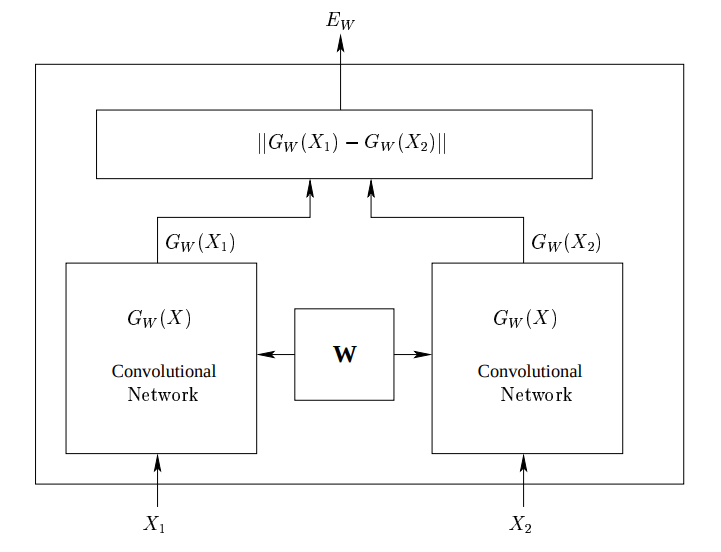
\includegraphics[width=0.8\linewidth]{siamese_architecture.png}
    \end{center}
    \caption{Siamese Architecture. (LeCun 2005)}
    \label{fig:siamese}
\end{figure}
I think LeCun proposed Contrastive Loss...\cite{LeCun}.
[Note: the partitioning and pairing of images is the same idea as SigNet.]
They did this on images of faces.

``A model is constructed of each subject by calculating the mean feature
vector and the variance-covariance matrix using the feature
vectors generated from the first five images of each subject.
The likelihood that a test image is genuine, $p_genuine$, is
found by evaluating the normal density of the test image on
the model of the concerned subject. The likelihood of a test
image being an impostor, $p_imposter$, is assumed to be a constant whose value is estimated by calculating the average $p_genuine$ value of all the impostor images of the concerned
subject. The probability that the given image is genuine is
given by P = $p_genuine$ / ($p_genuine$ + $p_imposter$)''
...so basically they assume that subjects/signers occupy a normal region in the latent space.

\subsection{Triplet Loss}
``FaceNet directly trains
its output to be a compact 128-D embedding using a triplet-based loss function based on LMNN [19]. Our triplets consist of two matching face thumbnails and a non-matching
face thumbnail and the loss aims to separate the positive pair
from the negative by a distance margin. The thumbnails are
tight crops of the face area, no 2D or 3D alignment, other
than scale and translation is performed.''
You could train a classifier and then take an intermediate layer to be a latent space, but this doesn't perform as well...
PCA can improve this, but an end-to-end network performs better.
\cite{face_net}

``The networks are trained by using a combination of classification and verification loss. The verification
loss is similar to the triplet loss we employ [12, 19], in that it
minimizes the L2-distance between faces of the same identity and enforces a margin between the distance of faces of
different identities. The main difference is that only pairs of
images are compared, whereas the triplet loss encourages a
relative distance constraint.''
``Although we did not directly compare to other losses,
e.g. the one using pairs of positives and negatives, as used
in [14] Eq. (2), we believe that the triplet loss is more suitable for face verification. The motivation is that the loss
from [14] encourages all faces of one identity to be projected onto a single point in the embedding space. The
triplet loss, however, tries to enforce a margin between each
pair of faces from one person to all other faces. This allows the faces for one identity to live on a manifold, while
still enforcing the distance and thus discriminability to other
identities.''
When training, they don't use true negatives to adjust weights because the network already knows they are different and so the direction of the gradient is somewhat arbitrary...
[Maybe I should try that...]
They just use a cut off threshold for computing accuracy.
I couldn't find how they chose the threshold...
Part of the results of their paper is that they conclude that using 256-bit over 128-bit latent vectos doesn't really improve accuracy.

\subseciton{asdf}
this paper (where FaceNet got triplet loss...) allows datapoints with the same label to live in multiple clusters:
https://proceedings.neurips.cc/paper/2005/file/a7f592cef8b130a6967a90617db5681b-Paper.pdf
Does FaceNet allow a subject/person to live in several clusters?
The FaceNet paper suggests that each person lives in a single cluster (they imply that and their verifyication strategy is just a distance threshold...)

\subsection{SigNet}
SigNet was largely inspired by the success of FaceNet.
I haven't seen the SigNet paper discuss why they didn't use triplet loss...

Yo, why does SigNet use contrastive loss instead of triplet loss?
    My guess is that Contrastive Loss is just easier to implement...
\cite{sig_net}
\cite{GitHub_sounakdey}
...and in python: \cite{GitHub_signet_pytorch}

\subsection{DeepFool}
\subsection{DEFENSE-GAN}

\subsection{FGSM}

